% Required packages: amsmath, amssymb, bm, graphicx
% Define \methodname before inputting this file if a different name is desired.
\providecommand{\methodname}{AdaPGC+}

\section{Method}
\label{sec:method}

\subsection{Problem Setup and Overview}
\label{sec:overview}

We consider source-free test-time adaptation for an audio--visual classifier.
At test time, either modality can be corrupted or entirely missing, and no
source data or target labels are available.  For a test sample, the frozen
backbone produces audio, video, and fused representations
$\bm z^{a},\bm z^{v},\bm z^{F}\in\mathbb{R}^{d}$ whenever the corresponding
views are observable.  We adapt only the first fusion-attention projections
and LayerNorm affine parameters, which keeps the update lightweight and limits
catastrophic drift.

As illustrated in Fig.~\ref{fig:framework}, \methodname has three components.
First, online class-conditional Gaussian models provide stable probabilistic
guidance for each representation.  Second, when one modality is missing, we
recover the distribution of the unavailable fused representation from the
observed modality.  Third, we detect the less reliable modality for each
sample and align only that branch, avoiding contamination of the reliable
branch.

\begin{figure*}[t]
  \centering
  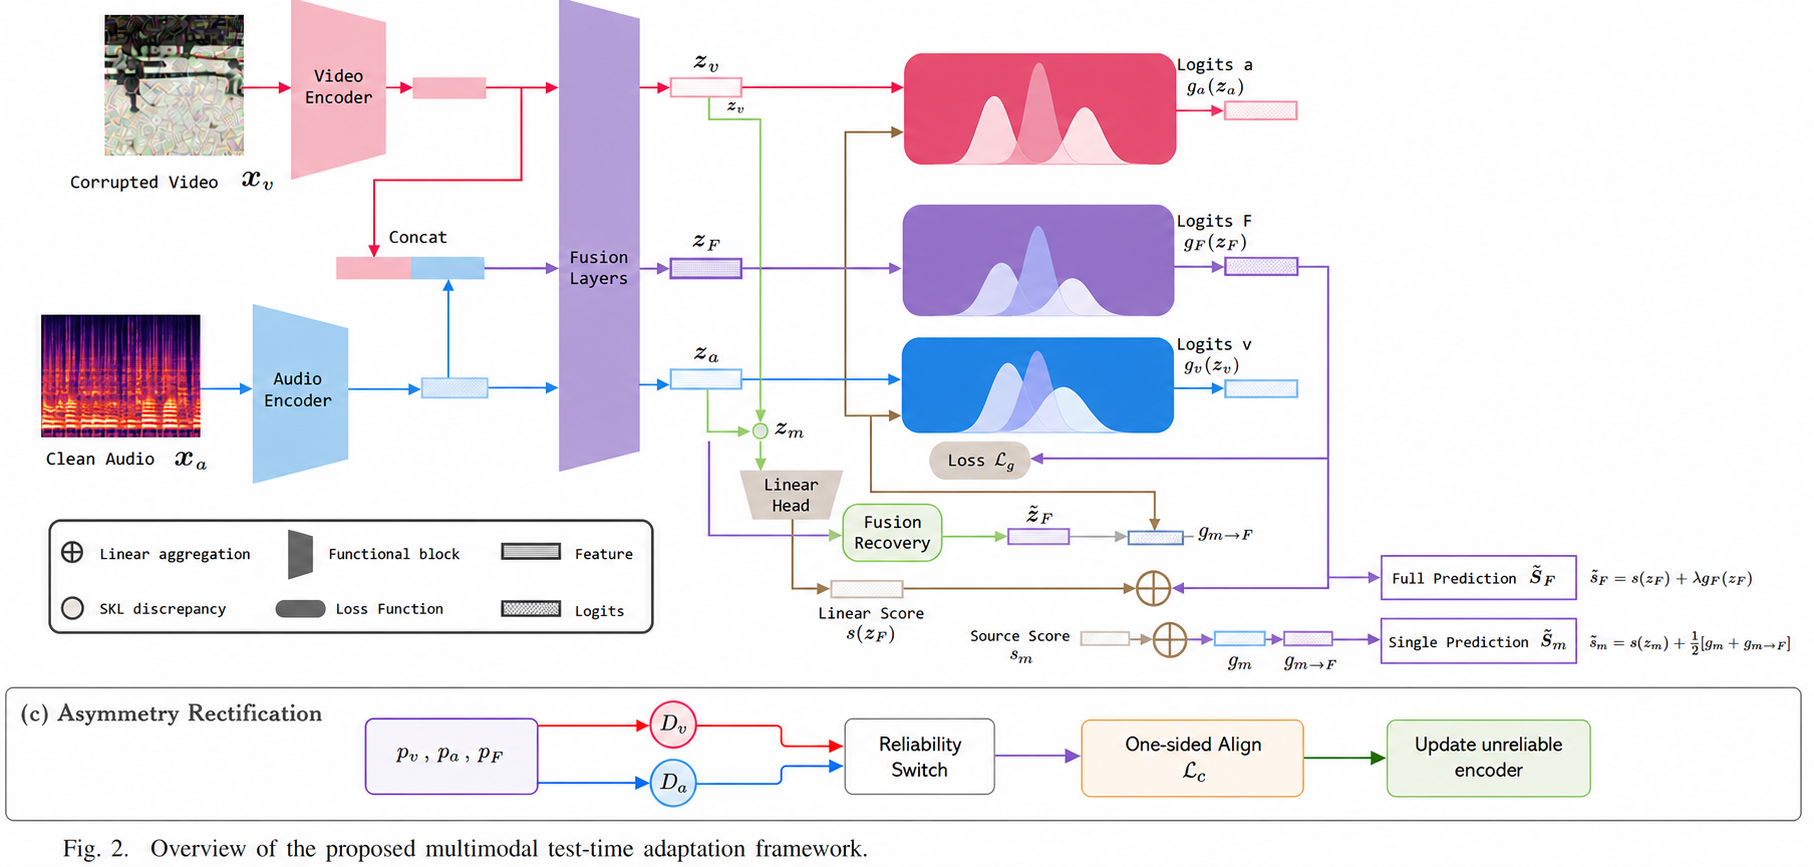
\includegraphics[width=0.99\textwidth,trim=0 35bp 0 0,clip]{adapgc_plus_framework_v5.png}
  \caption{Overview of \methodname. Online class-conditional Gaussian models
  guide prediction and adaptation. Fully observed samples update cross-view
  statistics; these statistics recover fused predictions when one modality is
  missing. A reliability switch performs one-sided cross-modal alignment.}
  \label{fig:framework}
\end{figure*}

\subsection{Online Probabilistic Guidance}
\label{sec:gmm}

\paragraph{Class-conditional modeling.}
For each view $r\in\{a,v,F\}$, we maintain an online Gaussian mixture with one
component per class:
\begin{equation}
  p_r(\bm z\mid y=c)=
  \mathcal{N}(\bm z;\bm\mu_c^r,\bm\Sigma_c^r),
  \qquad p_r(y=c)=\pi_c^r .
  \label{eq:gmm}
\end{equation}
Let the pretrained linear classifier be
$s_c(\bm z)=\bm w_c^{\top}\bm z+b_c$.  We initialize
$\bm\mu_c^r=\bm w_c$, $\bm\Sigma_c^r=\bm I$, and
\begin{equation}
  \pi_c^r\propto
  \exp\!\left(b_c+\tfrac{1}{2}\lVert\bm w_c\rVert_2^2\right),
  \label{eq:init}
\end{equation}
so the initial Gaussian discriminant is consistent with the source
classifier.  For each incoming batch, the network posterior
$q_{ic}=\operatorname{softmax}(\bm s_i)_c$ acts as a soft assignment.  We
update the effective count, first moment, and second moment online:
\begin{equation}
  \begin{aligned}
    \Delta N_c&=\sum_i q_{ic}, &
    \Delta\bm S_c&=\sum_i q_{ic}\bm z_i,\\
    \Delta\bm Q_c&=\sum_i q_{ic}\bm z_i\bm z_i^{\top}.
  \end{aligned}
  \label{eq:stats}
\end{equation}
and use exponential smoothing to obtain $\pi_c^r$, $\bm\mu_c^r$, and
$\bm\Sigma_c^r$.  This soft update uses every test sample while avoiding
hard pseudo-label errors.

The resulting Gaussian discriminant score is
\begin{equation}
  \begin{aligned}
  g_{r,c}(\bm z)={}&\log\pi_c^r-
  \tfrac{1}{2}\log|\bm\Sigma_c^r|\\
  &-\tfrac{1}{2}(\bm z-\bm\mu_c^r)^{\top}
  (\bm\Sigma_c^r)^{-1}(\bm z-\bm\mu_c^r),
  \end{aligned}
  \label{eq:gda}
\end{equation}
where class-independent constants are omitted.

\paragraph{Guided adaptation.}
Let $\bm g_i$ denote the probabilistic score selected according to the
sample's available modalities; its missing-modality form is defined below.
We transfer this distribution to the network with
\begin{equation}
  \begin{aligned}
  \mathcal{L}_{g}&=-\frac{1}{B}\sum_{i=1}^{B}
  \sum_{c=1}^{C}p^g_{ic}\log p^{\theta}_{ic},\\
  \bm p_i^g&=\operatorname{softmax}(\bm g_i),\qquad
  \bm p_i^{\theta}=\operatorname{softmax}(\bm s_i).
  \end{aligned}
  \label{eq:guidance}
\end{equation}
Only the query, key, and value projections in the first fusion-attention
block are updated by this loss.

\subsection{Conditional Fusion Recovery}
\label{sec:recovery}

Prediction from a single observed modality is weaker because the fused
representation is unavailable.  We therefore estimate the class-wise
cross-covariance $\bm\Sigma_c^{mF}=\operatorname{Cov}(\bm z^m,\bm z^F\mid
y=c)$ from fully observed test samples, where $m\in\{a,v\}$.  These statistics
are updated online with the same soft assignments as Eq.~\eqref{eq:stats}.

Given an observed feature $\bm z^m$ and a possible class $c$, Gaussian
conditioning yields a recovered fused mean
\begin{equation}
  \widehat{\bm z}_{c}^{F\mid m}=
  \bm\mu_c^F+
  (\bm\Sigma_c^{mF})^{\top}(\bm\Sigma_c^m)^{-1}
  (\bm z^m-\bm\mu_c^m).
  \label{eq:conditional_mean}
\end{equation}
Because $c$ is unknown, we compute a soft class responsibility from the
observed view,
\begin{equation}
  \alpha_c^m=
  \operatorname{softmax}\!\left(\bm g_m(\bm z^m)/T\right)_c,
  \label{eq:responsibility}
\end{equation}
score every conditional recovery with the fused-view discriminator, and
marginalize over the recovery class:
\begin{equation}
  g_{m\rightarrow F,k}(\bm z^m)=
  \sum_{c=1}^{C}\alpha_c^m\,
  g_{F,k}\!\left(\widehat{\bm z}_{c}^{F\mid m}\right).
  \label{eq:recovery_score}
\end{equation}
Thus, the method does not commit to a single pseudo-label during recovery.
The final probabilistic guidance is
\begin{equation}
  \bm g_i=
  \begin{cases}
    \bm g_F(\bm z_i^F), & \text{full},\\
    (1-\beta)\bm g_{m\rightarrow F}(\bm z_i^m)
    +\beta\bm g_m(\bm z_i^m), & \text{$m$ only}.
  \end{cases}
  \label{eq:guidance_cases}
\end{equation}
Before enough paired samples have been accumulated, we safely fall back to
$\bm g_m(\bm z^m)$.

\subsection{Asymmetry Rectification}
\label{sec:rectification}

When both modalities are present, corruption is often asymmetric: forcing the
two branches to learn from each other equally can degrade the cleaner branch.
For each sample, we compare each unimodal prediction with the fused prediction
using symmetric KL divergence,
\begin{equation}
  D_m=\tfrac{1}{2}\left[
  \operatorname{KL}(\bm p_F\|\bm p_m)+
  \operatorname{KL}(\bm p_m\|\bm p_F)\right],
  \qquad m\in\{a,v\}.
  \label{eq:reliability}
\end{equation}
The modality with the smaller $D_m$ is treated as the reliable target, while
the other modality is updated.  Let $r_i$ and $u_i$ be the reliable and
unreliable modalities for sample $i$.  We use the one-sided contrastive loss
\begin{equation}
  \mathcal{L}_{c}=-\frac{1}{|\mathcal{I}|}
  \sum_{i\in\mathcal{I}}
  \log\frac{
  \exp\!\left(\operatorname{sim}(\bm z_i^{u_i},
  \operatorname{sg}(\bm z_i^{r_i}))/\tau\right)}{
  \sum_j\exp\!\left(\operatorname{sim}(\bm z_i^{u_i},
  \operatorname{sg}(\bm z_j^{r_i}))/\tau\right)},
  \label{eq:contrastive}
\end{equation}
where $\operatorname{sg}(\cdot)$ stops the gradient.  Consequently, only the
unreliable representation is pulled toward the reliable one.  This loss
updates the LayerNorm affine parameters and is applied only to fully observed
samples.

\subsection{Online Update and Prediction}
\label{sec:optimization}

The two parameter groups are optimized separately:
\begin{equation}
  \mathcal{L}_{\mathrm{fusion}}=
  \lambda_g\mathcal{L}_g+\lambda_b\mathcal{L}_{\mathrm{base}},
  \qquad
  \mathcal{L}_{\mathrm{LN}}=\lambda_c\mathcal{L}_c,
  \label{eq:objective}
\end{equation}
where $\mathcal{L}_{\mathrm{base}}$ is an optional entropy-and-diversity
regularizer and can be disabled.  We maintain an exponential moving average
$\bar\theta$ of the adapted network.  The final prediction combines its logits
with the probabilistic guidance:
\begin{equation}
  \widetilde{\bm s}_i=\bm s_{\bar\theta}(\bm x_i)+\gamma\bm g_i,
  \qquad
  \widehat y_i=\arg\max_c\widetilde s_{i,c}.
  \label{eq:final_prediction}
\end{equation}
All statistics and parameters are updated once per arriving batch; no target
labels, source samples, or offline retraining are required.
